\documentclass[9pt,twoside]{pnas-new}

\templatetype{pnasmathematics} % one-column template
\setboolean{displaywatermark}{false}

\usepackage{graphicx}
\usepackage[T1]{fontenc}
\usepackage[utf8]{inputenc}
\begin{document}

\title{Reproduction and Extension of an Agent-Based Sheep-Herding Model}

\author[a]{Anja Pijak}
\author[a]{Ana Nikolić}
\author[a]{Mia Miletić}
\author[a]{Kristina \DJ uki\'c}

\affil[a]{Faculty of Computer and Information Science, University of Ljubljana, Slovenia}

\leadauthor{Pijak}

\significancestatement{Animal groups such as sheep flocks move coherently although each animal reacts only to its neighbours and to nearby threats. We reproduce a recent model of sheep responding to a herding dog and propose a fuzzy-logic extension in which each sheep responds to the dog in a graded, individual way, testing whether differences between animals change the motion of the whole flock.}

% \authorcontributions{TODO: add the contribution of each author.}
% \authordeclaration{The authors declare no competing interests.}
% \correspondingauthor{To whom correspondence should be addressed. E-mail: ap72051@student.uni-lj.si}

\keywords{Collective Behaviour $|$ Agent-Based Modelling $|$ Sheep Herding $|$ Fuzzy Logic $|$ Simulation}

\begin{abstract}
Collective behaviour emerges from local interactions among individuals, and herding provides a controlled setting in which to study how information propagates through a group. We build on the agent-based model of Jadhav et al.\ (2024), in which 14 sheep respond to a herding dog through repulsion, attraction, alignment, persistence, noise, and dog avoidance. As a baseline, we reimplemented the published MATLAB model in Python and analysed three flock-level measures (polarization, cohesion, elongation) and five measures describing the position and motion of the dog relative to the flock. A 300-run Python baseline, matching the ensemble size of the original code, produces qualitatively similar results to the original MATLAB implementation and closely matches the flock-level distributions reported by Jadhav et al. Some dog-related distributions, particularly the relative-angle distributions, differ quantitatively from the published figures, even when generated using the original MATLAB implementation. The implementations have been compared using descriptive statistics, but formal statistical testing remains to be performed. Building on this baseline, we propose a single extension: replacing the fixed dog-avoidance response of each sheep by a fuzzy inference system that maps the dog's distance to an avoidance intensity, with sheep differing in sensitivity. Three scenarios (original, homogeneous fuzzy, heterogeneous fuzzy) will be compared across many random seeds to separate the effect of graded responses from the effect of individual differences.
\end{abstract}

\dates{This manuscript was compiled on \today}

\maketitle
\thispagestyle{firststyle}
\ifthenelse{\boolean{shortarticle}}{\ifthenelse{\boolean{singlecolumn}}{\abscontentformatted}{\abscontent}}{}

\Firstpage

\section{Introduction}

Groups of animals, from insect swarms to fish schools and sheep flocks, often move as a coherent whole although no individual has a global view of the group. Such coordination arises from simple local interactions, and the central question of collective behaviour research is how rules acting on individuals give rise to group-level patterns \cite{sumpter2006}. Three interaction types recur in most models: repulsion at short range, which prevents collisions; attraction at longer range, which keeps the group together; and alignment, in which an individual adjusts its heading to that of its neighbours \cite{reynolds1987,couzin2002}.

Vicsek et al.\ \cite{vicsek1995} showed that alignment alone is sufficient to produce collective motion: self-propelled particles that adopt the average heading of their neighbours, perturbed by noise, undergo a transition from disordered motion to global order as noise decreases or density increases.

Herding adds an external agent that actively shapes the group. Str\"{o}mbom et al.\ \cite{strombom2014} proposed a heuristic model of the shepherding problem in which a single herder alternates between two behaviours depending on the flock's state: \emph{collecting}, in which it moves behind the stray sheep furthest from the flock to bring it back, and \emph{driving}, in which it moves behind a compact flock to push it towards a target. The sheep follow repulsion, attraction and a response to the herder, and the model shows that two simple herder rules suffice to control the flock.

Jadhav et al.\ \cite{jadhav2024} tested these ideas against data. They tracked 14 sheep and a border collie during 26 herding activities and analysed how information about a change of direction spreads through the flock, quantifying cohesion, polarization, elongation, and the position of the dog relative to the flock. They then proposed an agent-based model, extending earlier shepherding models, that reproduces the observed statistics. We chose it because it is empirically grounded and fully specified, with public code, which makes a faithful reproduction feasible.

In the Jadhav model all sheep respond to the dog identically: a fixed avoidance coefficient is applied whenever the dog is within a fixed radius. Real animals differ in boldness, perception, and reaction time, and a graded response to proximity is more plausible than a hard threshold. Fuzzy logic provides a natural way to express such graded responses through linguistic categories with smooth transitions \cite{zadeh1965}. It has also been applied to modelling collective animal behaviour, including flocking simulations \cite{lebarbajec2005}. It is therefore unclear how much of the observed flock-level behaviour depends on the homogeneous, thresholded response. We ask:

\begin{quote}
\emph{How does a graded, individually heterogeneous response to the herding dog, modelled with fuzzy logic, change the collective stability and movement of a sheep flock compared with the original homogeneous model?}
\end{quote}

\section{Methods}

\subsection{Baseline model}
The baseline follows the agent-based model of Jadhav et al.\ \cite{jadhav2024}. $N=14$ sheep and one dog move in a square arena of side 250 for 370 discrete time steps. Each sheep updates its velocity from a weighted sum of components: persistence of its previous heading (coefficient 0.5), repulsion from sheep closer than 2 units, attraction towards the centre of 4 neighbours selected from its 10 nearest (weight 1.5), alignment with 1 selected neighbour (weight 1.3), and a random component (coefficient 0.3). When the dog is within a radius of 12 units, the sheep additionally avoids the dog with weight $\rho_d=1.0$; outside this radius, only repulsion from other sheep and persistence apply. Sheep move at speed 1.0 and the dog at 1.5.

The dog switches between three modes. When the flock is dispersed, it \emph{collects}: it moves towards a point behind the sheep that is furthest from the flock centre. When the flock is compact, it \emph{drives}: it moves to a position behind the flock centre. When it comes too close to a sheep, it \emph{slows down}, reducing its speed from 1.5 to 0.05.

\subsection{Python implementation}
The model was reimplemented in Python (NumPy), with the number of independent runs and the random seed as inputs. Unit checks verify that exactly one dog mode is active per step, that dog speeds equal 1.5 or 0.05, and that all positions are finite. All parameters, including the collecting and driving thresholds, were checked against the original MATLAB code, which uses 300 independent runs of 370 steps, and against the supplementary information of \cite{jadhav2024}.

One implementation detail deserves mention. In the published MATLAB code, when a single alignment neighbour is used ($n_\mathrm{Ali}=1$), the neighbour's velocity is a $1\times2$ row vector and the \texttt{sum} function adds its two components into a scalar before normalisation. Our Python code reproduces this behaviour deliberately. It therefore follows the published code, but for $n_\mathrm{Ali}=1$ it is not identical to the vectorial alignment described in the text of the paper. We kept it so that the baseline remains comparable with the original, and we will test its effect in the evaluation phase.

\subsection{Metrics}
Following \cite{jadhav2024}, we compute eight measures. Three describe the flock. \emph{Polarization} measures alignment of headings,
\begin{equation}
P(t)=\left|\frac{1}{N}\sum_{i=1}^{N}\frac{\mathbf{v}_i(t)}{|\mathbf{v}_i(t)|}\right|\in[0,1],
\end{equation}
\emph{cohesion} is the mean distance of the sheep from the flock centre, and \emph{elongation} is the ratio of the flock's extent along its mean heading to its extent perpendicular to it, so that values above 1 indicate a flock stretched in the direction of motion. Five measures describe the dog relative to the flock: the distance of the dog from the rearmost sheep, its lateral offset from the flock, and three signed angles: $\psi_{BD}$, between the flock's mean heading and the vector from the flock centre to the dog; $\psi_{DB}$, between the dog's heading and the vector from the dog to the flock centre; and $\phi_{BD}$, between the flock's mean heading and the dog's heading. For each measure we estimate the probability density function over all time steps and runs. Angular quantities are summarised here by their median, since the arithmetic mean of angles near $\pm180^\circ$ is not meaningful; circular statistics will be used in later analyses.

\subsection{Planned extension: fuzzy individual responsiveness}
We select a single extension and leave other directions (e.g.\ the direction from which the dog approaches, or multiple dogs) for future work. In the original model the avoidance of the dog is a fixed-weight term applied inside a hard radius. We will replace the weight by the output of a Mamdani fuzzy inference system \cite{zadeh1965,mamdani1975}, leaving all other sheep rules and the dog strategy unchanged.

The system has one input, the distance $d_i$ between sheep $i$ and the dog, with linguistic terms \emph{far}, \emph{medium}, and \emph{near}, and one output, the avoidance intensity $\rho_i$, with terms \emph{weak}, \emph{moderate}, and \emph{strong}. The rule base has three rules: IF the dog is far THEN avoidance is weak; IF the dog is at medium distance THEN avoidance is moderate; IF the dog is near THEN avoidance is strong. The crisp output, obtained by centroid defuzzification, replaces $\rho_d$ in the avoidance term of sheep $i$.

Individual differences are introduced through sensitivity profiles: each sheep is assigned one of three profiles (low, medium, high sensitivity) that shifts the membership functions of its input, so that a high-sensitivity sheep perceives the same distance as ``nearer''. The shapes and parameters of the membership functions will be defined in the next phase of the project, based on the range of dog--sheep distances observed in the baseline simulations, and their influence will be assessed in a sensitivity analysis. We deliberately restrict the first version to one input, one output, and three profiles, so that effects can be attributed to a single mechanism.

\subsection{Experimental design}
Three scenarios will be compared: \textbf{A}, the original model with identical, fixed avoidance (baseline); \textbf{B}, the fuzzy model with the same fuzzy system for all sheep (isolates the effect of graded responses); and \textbf{C}, the fuzzy model with heterogeneous sensitivity profiles (main extension). Each scenario will be run with the same set of random seeds and the same number of runs, and all eight measures will be compared. Because time steps within a run are correlated, the measures will be summarised per run, and the scenarios will be compared across independent runs rather than across individual time steps. 

\section{Results}

\subsection{Python baseline}
We ran 300 independent Python simulations (seed 42, 370 steps each; 111\,000 time steps in total). Table~\ref{tab:stats} summarises the eight measures. The flock is moderately polarized (median 0.87) and cohesive (mean distance from the centre about 3 units), and elongation is slightly below 1 (median 0.82), i.e.\ the flock is marginally wider than it is long. The dog drives for about 91\% of the time, collects for about 7\%, and slows down for about 2\%. The dog is typically positioned behind the rearmost sheep (median distance 2.7 units), while $\psi_{DB}$ and $\phi_{BD}$ are concentrated near $0^\circ$ (medians $2.4^\circ$ and $-0.1^\circ$).

% Values below come from python_baseline_300.npz (analysis.py and dog_metrics.py, --runs 300 --seed 42).
\begin{table}[t!]
\centering
\caption{Summary statistics of the Python baseline (300 runs, seed 42, 370 steps; $n=111\,000$ samples per measure, $110\,700$ for angles). Means are omitted for angles.}
\label{tab:stats}
\begin{tabular}{lrr}
Measure & Mean & Median \\
\midrule
Polarization & 0.77 & 0.87 \\
Cohesion & 3.22 & 3.04 \\
Elongation & 0.91 & 0.82 \\
Dog to rearmost sheep & 2.16 & 2.69 \\
Dog lateral offset & 0.23 & 0.49 \\
$\psi_{BD}$ ($^\circ$) & -- & $-118.9$ \\
$\psi_{DB}$ ($^\circ$) & -- & 2.4 \\
$\phi_{BD}$ ($^\circ$) & -- & $-0.1$ \\
\bottomrule
\end{tabular}
\end{table}

\subsection{Comparison with the original results}
The flock-level distributions of polarization, cohesion, and elongation closely match those reported in the original study \cite{jadhav2024}. For the dog-related measures, MATLAB and Python give very similar distributions: the dog is mostly behind the rearmost sheep, its lateral displacement is broad and flat, $\psi_{BD}$ concentrates near $\pm180^\circ$, and $\phi_{BD}$ peaks narrowly near $0^\circ$. However, three of these distributions (distance to the rearmost sheep, lateral displacement, and the angles) differ visibly from the published ones for both implementations, so the cause of the mismatch remains open. The comparison is visual only: the random number generators differ, and no statistical test has been applied yet. All figures are available in the project repository.

% Optional figure (needs figs/ files; check the 4-page limit before enabling):
%\begin{figure}[t!]
%\centering
%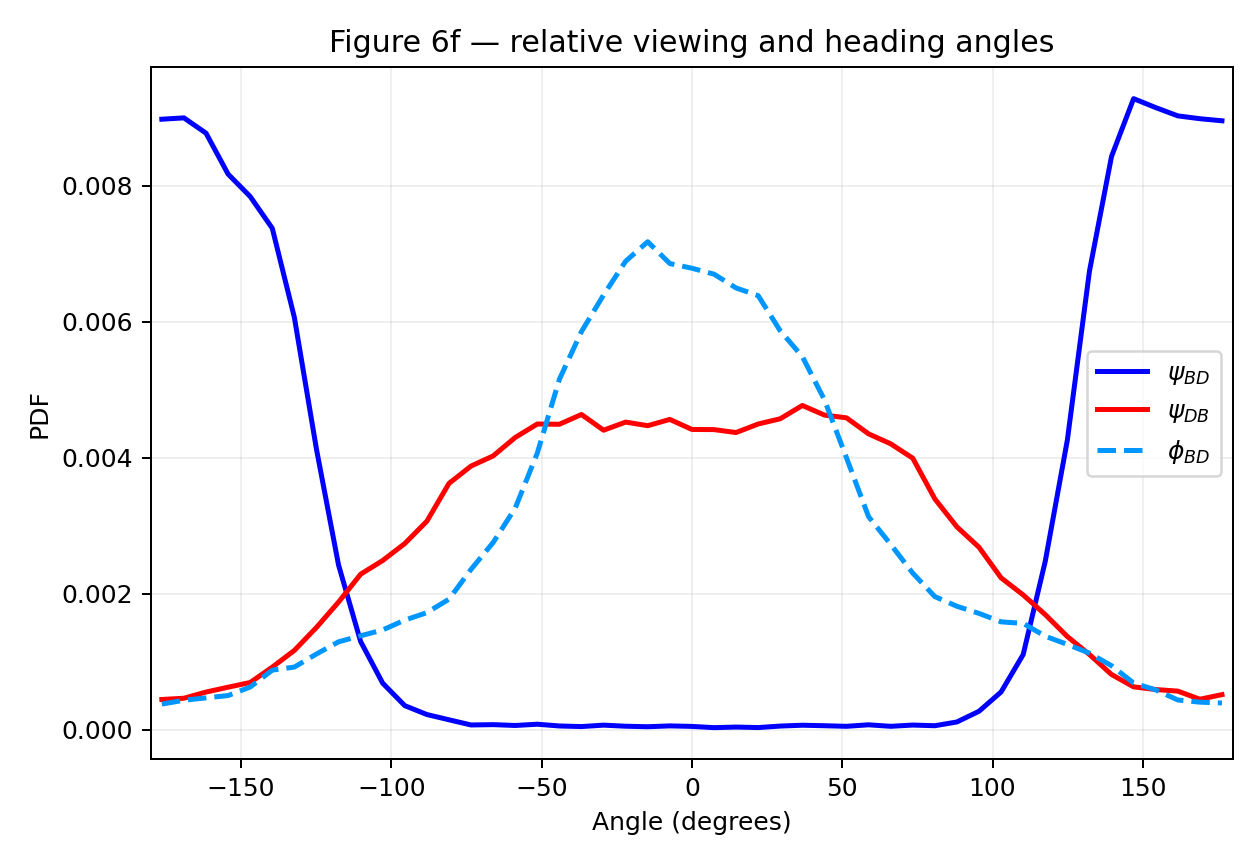
\includegraphics[width=0.4\linewidth]{figs/figure_6f_angles_matlab.png}
%\hspace{0.03\linewidth}
%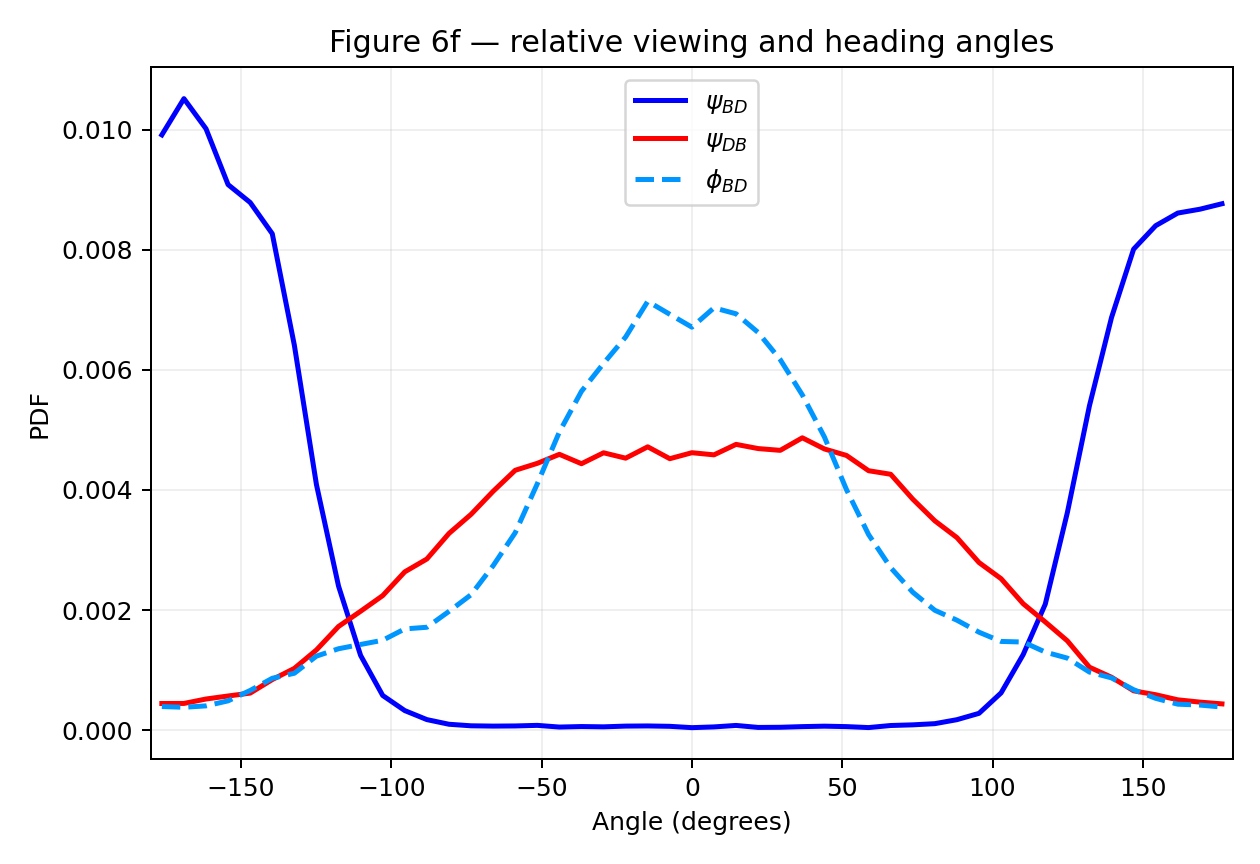
\includegraphics[width=0.4\linewidth]{figs/figure_6f_angles.png}
%\caption{Distributions of $\psi_{BD}$, $\psi_{DB}$ and $\phi_{BD}$ for the MATLAB (left) and Python (right) implementations, 300 runs each.}
%\label{fig:angles}
%\end{figure}


\section{Discussion}

Our baseline reproduces the main qualitative features of the Jadhav model: a cohesive, polarized flock whose distributions match the original, and a dog that mostly drives from behind and occasionally collects stragglers. The reproduction is not yet fully validated. Three dog-related distributions differ from the published figures in both implementations. Since the MATLAB and Python results are qualitatively similar, the discrepancy is unlikely to be caused solely by our Python implementation, but its origin remains unclear. We will check whether it arises from parameters that differ from the Supplementary Table of \cite{jadhav2024}, from different code versions in the original repository, or from how the published distributions were computed (e.g.\ which time steps were analysed). Moreover, the comparison is visual, and the retained scalar alignment means that agreement with MATLAB shows fidelity to the code rather than to the model described in the paper. In the next phase, we will compare run-level summaries across independent simulations, using appropriate statistical methods for each measure, including circular statistics for angular quantities.

The proposed extension targets an assumption of the original model that is biologically unrealistic but rarely examined: that all sheep respond to the dog identically and abruptly. By including scenario B, we can distinguish the effect of graded responses from the effect of heterogeneity, which would be confounded if only scenario C were studied. We expect that moderate heterogeneity may lead to earlier reactions among sensitive sheep, whereas strong heterogeneity may reduce polarization and cohesion as less sensitive sheep respond later and the flock stretches. These are hypotheses, not findings, and the outcome may well be that the flock is robust to such variation, which would itself be informative.

The design has limitations. The shapes and breakpoints of the membership functions are design choices; we will report a sensitivity analysis over them rather than a single tuned configuration. Using the distance to the dog as the only input ignores the dog's speed and approach angle. Finally, simulated heterogeneity is not calibrated against real sheep, so conclusions concern the mechanism rather than the animals. Natural follow-ups include varying the direction of the dog's approach and introducing multiple dogs.

\dataavail{Code, LaTeX source, and the PDF of this report are available at \url{https://github.com/dolouress/collective-behaviour-groupD}.}

% \showacknow

\bibliography{references}

\end{document}